\documentclass[border=8pt]{standalone}
\usepackage{amsmath,amssymb}
\usepackage{tikz}
\usetikzlibrary{arrows.meta,backgrounds,calc,fit,positioning}

\definecolor{paperpink}{HTML}{F4DADA}
\definecolor{paperlavender}{HTML}{E9E4F1}
\definecolor{papergreen}{HTML}{DDECDD}
\definecolor{paperyellow}{HTML}{F5F2C8}
\definecolor{paperpeach}{HTML}{FBEBD6}
\definecolor{paperblue}{HTML}{E2ECF4}
\definecolor{ink}{HTML}{252525}
\definecolor{rulegray}{HTML}{9A9A9A}

\begin{document}
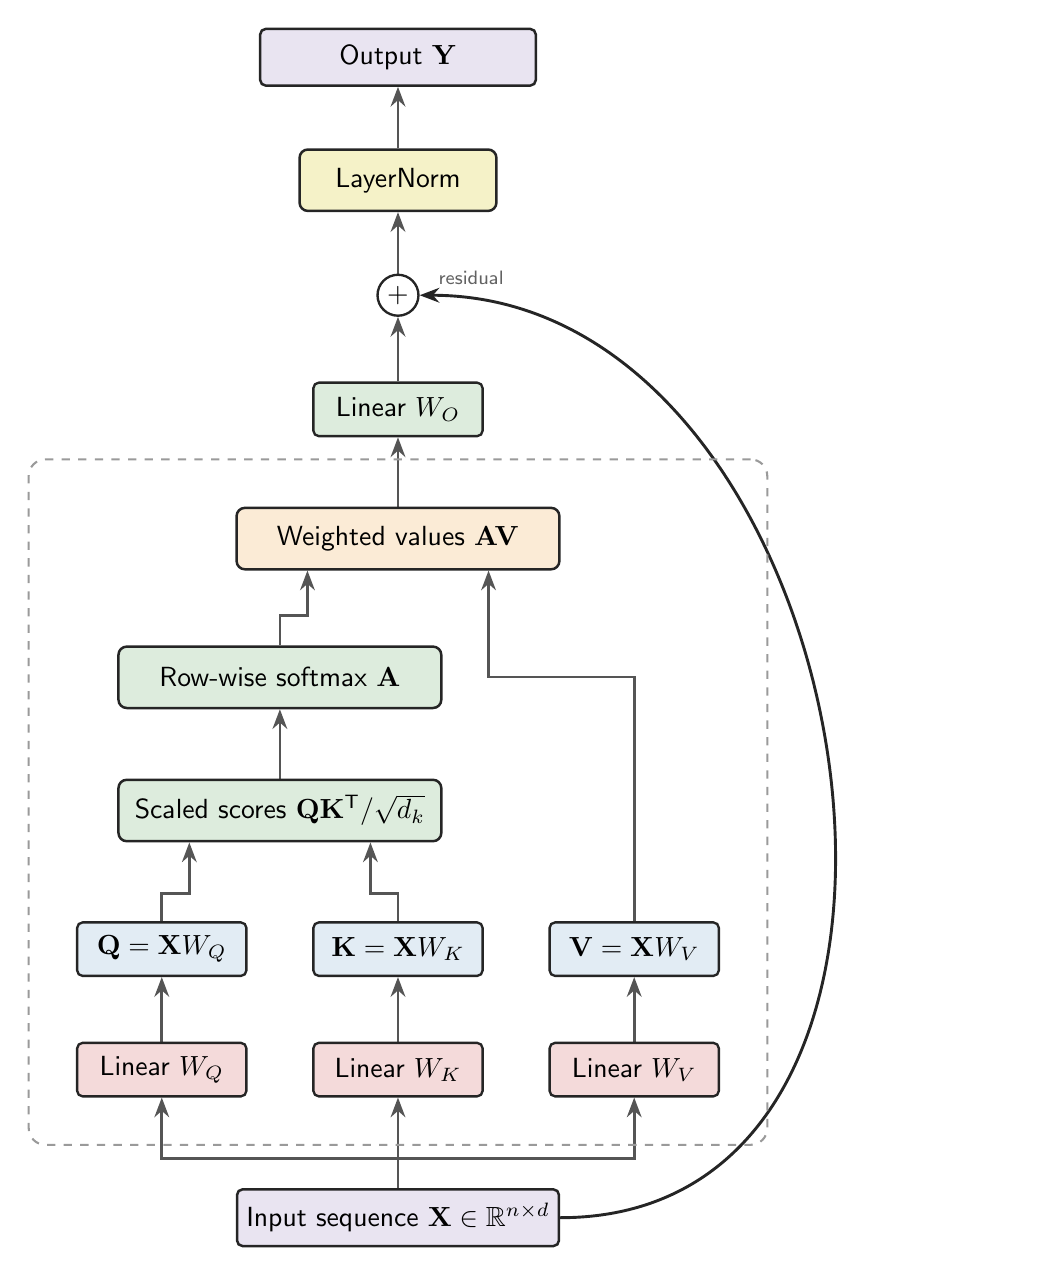
\begin{tikzpicture}[
  >={Stealth[length=2.5mm]},
  font=\sffamily,
  state/.style={draw=ink,fill=paperlavender,rounded corners=2pt,line width=.9pt,minimum width=3.5cm,minimum height=.72cm,align=center},
  proj/.style={draw=ink,fill=paperpink,rounded corners=2pt,line width=.85pt,minimum width=2.15cm,minimum height=.68cm,align=center},
  outproj/.style={draw=ink,fill=papergreen,rounded corners=2pt,line width=.85pt,minimum width=2.15cm,minimum height=.68cm,align=center},
  tensor/.style={draw=ink,fill=paperblue,rounded corners=2pt,line width=.85pt,minimum width=2.15cm,minimum height=.68cm,align=center},
  compute/.style={draw=ink,fill=papergreen,rounded corners=3pt,line width=.9pt,minimum width=4.1cm,minimum height=.78cm,align=center},
  attention/.style={draw=ink,fill=paperpeach,rounded corners=3pt,line width=.9pt,minimum width=4.1cm,minimum height=.78cm,align=center},
  norm/.style={draw=ink,fill=paperyellow,rounded corners=3pt,line width=.9pt,minimum width=2.5cm,minimum height=.78cm,align=center},
  merge/.style={circle,draw=ink,line width=.85pt,fill=white,minimum size=.52cm,inner sep=0pt},
  flow/.style={draw=ink!78,line width=.95pt,->},
  residual/.style={draw=ink,line width=1.05pt,->},
  group/.style={draw=rulegray,dashed,rounded corners=6pt,line width=.75pt,inner sep=6mm},
  label/.style={font=\sffamily\scriptsize,text=ink!72}
]
  \node[state] (input) {Input sequence $\mathbf{X}\in\mathbb{R}^{n\times d}$};

  \node[proj,above=1.15cm of input,xshift=-3.0cm] (qproj) {Linear $W_Q$};
  \node[proj,above=1.15cm of input] (kproj) {Linear $W_K$};
  \node[proj,above=1.15cm of input,xshift=3.0cm] (vproj) {Linear $W_V$};

  \node[tensor,above=.82cm of qproj] (q) {$\mathbf{Q}=\mathbf{X}W_Q$};
  \node[tensor,above=.82cm of kproj] (k) {$\mathbf{K}=\mathbf{X}W_K$};
  \node[tensor,above=.82cm of vproj] (v) {$\mathbf{V}=\mathbf{X}W_V$};

  \node[compute,above=1.0cm of k,xshift=-1.5cm] (score) {Scaled scores $\mathbf{Q}\mathbf{K}^{\mathsf T}/\sqrt{d_k}$};
  \node[compute,above=.88cm of score] (softmax) {Row-wise softmax $\mathbf{A}$};
  \node[attention,above=.95cm of softmax,xshift=1.5cm] (mix) {Weighted values $\mathbf{A}\mathbf{V}$};
  \node[outproj,above=.88cm of mix] (outproj) {Linear $W_O$};
  \node[merge,above=.82cm of outproj] (add) {$+$};
  \node[norm,above=.78cm of add] (norm) {LayerNorm};
  \node[state,above=.78cm of norm] (output) {Output $\mathbf{Y}$};

  \begin{scope}[on background layer]
    \draw[flow] (input.north) -- ++(0,.38) -| (qproj.south);
    \draw[flow] (input.north) -- (kproj.south);
    \draw[flow] (input.north) -- ++(0,.38) -| (vproj.south);
    \draw[flow] (qproj) -- (q);
    \draw[flow] (kproj) -- (k);
    \draw[flow] (vproj) -- (v);
    \draw[flow] (q.north) -- ++(0,.35) -| ([xshift=-1.15cm]score.south);
    \draw[flow] (k.north) -- ++(0,.35) -| ([xshift=1.15cm]score.south);
    \draw[flow] (score) -- (softmax);
    \draw[flow] (softmax.north) -- ++(0,.38) -| ([xshift=-1.15cm]mix.south);
    \draw[flow] (v.north) -- ++(0,3.1) -| ([xshift=1.15cm]mix.south);
    \draw[flow] (mix) -- (outproj);
    \draw[flow] (outproj) -- (add);
    \draw[flow] (add) -- (norm);
    \draw[flow] (norm) -- (output);
    \draw[residual] (input.east) .. controls +(5.7,0) and +(5.7,0) .. (add.east);
  \end{scope}

  \node[label,anchor=south west,fill=white,inner sep=1pt] at ([xshift=2mm,yshift=1mm]add.east) {residual};
  \node[group,fit=(qproj)(vproj)(q)(v)(score)(softmax)(mix),label={[label]above:{Self-attention: $Q,K,V$ share the same source}}] {};
\end{tikzpicture}
\end{document}

